\documentclass[12pt,british,a4paper,]{article}
\usepackage{lmodern}
\usepackage{amssymb,amsmath}
\usepackage{ifxetex,ifluatex}
\usepackage{fixltx2e} % provides \textsubscript
\ifnum 0\ifxetex 1\fi\ifluatex 1\fi=0 % if pdftex
  \usepackage[T1]{fontenc}
  \usepackage[utf8]{inputenc}
\else % if luatex or xelatex
  \ifxetex
    \usepackage{mathspec}
  \else
    \usepackage{fontspec}
  \fi
  \defaultfontfeatures{Ligatures=TeX,Scale=MatchLowercase}
    \setmainfont[]{Calibri}
\fi
% use upquote if available, for straight quotes in verbatim environments
\IfFileExists{upquote.sty}{\usepackage{upquote}}{}
% use microtype if available
\IfFileExists{microtype.sty}{%
\usepackage{microtype}
\UseMicrotypeSet[protrusion]{basicmath} % disable protrusion for tt fonts
}{}
\usepackage[margin=2.5cm]{geometry}
\usepackage{hyperref}
\hypersetup{unicode=true,
            pdftitle={ThermStats : an R package for quantifying surface thermal heterogeneity in assessments of microclimates},
            pdfborder={0 0 0},
            breaklinks=true}
\urlstyle{same}  % don't use monospace font for urls
\ifnum 0\ifxetex 1\fi\ifluatex 1\fi=0 % if pdftex
  \usepackage[shorthands=off,main=british]{babel}
\else
  \usepackage{polyglossia}
  \setmainlanguage[variant=british]{english}
\fi
\usepackage{color}
\usepackage{fancyvrb}
\newcommand{\VerbBar}{|}
\newcommand{\VERB}{\Verb[commandchars=\\\{\}]}
\DefineVerbatimEnvironment{Highlighting}{Verbatim}{commandchars=\\\{\}}
% Add ',fontsize=\small' for more characters per line
\usepackage{framed}
\definecolor{shadecolor}{RGB}{248,248,248}
\newenvironment{Shaded}{\begin{snugshade}}{\end{snugshade}}
\newcommand{\AlertTok}[1]{\textcolor[rgb]{0.94,0.16,0.16}{#1}}
\newcommand{\AnnotationTok}[1]{\textcolor[rgb]{0.56,0.35,0.01}{\textbf{\textit{#1}}}}
\newcommand{\AttributeTok}[1]{\textcolor[rgb]{0.77,0.63,0.00}{#1}}
\newcommand{\BaseNTok}[1]{\textcolor[rgb]{0.00,0.00,0.81}{#1}}
\newcommand{\BuiltInTok}[1]{#1}
\newcommand{\CharTok}[1]{\textcolor[rgb]{0.31,0.60,0.02}{#1}}
\newcommand{\CommentTok}[1]{\textcolor[rgb]{0.56,0.35,0.01}{\textit{#1}}}
\newcommand{\CommentVarTok}[1]{\textcolor[rgb]{0.56,0.35,0.01}{\textbf{\textit{#1}}}}
\newcommand{\ConstantTok}[1]{\textcolor[rgb]{0.00,0.00,0.00}{#1}}
\newcommand{\ControlFlowTok}[1]{\textcolor[rgb]{0.13,0.29,0.53}{\textbf{#1}}}
\newcommand{\DataTypeTok}[1]{\textcolor[rgb]{0.13,0.29,0.53}{#1}}
\newcommand{\DecValTok}[1]{\textcolor[rgb]{0.00,0.00,0.81}{#1}}
\newcommand{\DocumentationTok}[1]{\textcolor[rgb]{0.56,0.35,0.01}{\textbf{\textit{#1}}}}
\newcommand{\ErrorTok}[1]{\textcolor[rgb]{0.64,0.00,0.00}{\textbf{#1}}}
\newcommand{\ExtensionTok}[1]{#1}
\newcommand{\FloatTok}[1]{\textcolor[rgb]{0.00,0.00,0.81}{#1}}
\newcommand{\FunctionTok}[1]{\textcolor[rgb]{0.00,0.00,0.00}{#1}}
\newcommand{\ImportTok}[1]{#1}
\newcommand{\InformationTok}[1]{\textcolor[rgb]{0.56,0.35,0.01}{\textbf{\textit{#1}}}}
\newcommand{\KeywordTok}[1]{\textcolor[rgb]{0.13,0.29,0.53}{\textbf{#1}}}
\newcommand{\NormalTok}[1]{#1}
\newcommand{\OperatorTok}[1]{\textcolor[rgb]{0.81,0.36,0.00}{\textbf{#1}}}
\newcommand{\OtherTok}[1]{\textcolor[rgb]{0.56,0.35,0.01}{#1}}
\newcommand{\PreprocessorTok}[1]{\textcolor[rgb]{0.56,0.35,0.01}{\textit{#1}}}
\newcommand{\RegionMarkerTok}[1]{#1}
\newcommand{\SpecialCharTok}[1]{\textcolor[rgb]{0.00,0.00,0.00}{#1}}
\newcommand{\SpecialStringTok}[1]{\textcolor[rgb]{0.31,0.60,0.02}{#1}}
\newcommand{\StringTok}[1]{\textcolor[rgb]{0.31,0.60,0.02}{#1}}
\newcommand{\VariableTok}[1]{\textcolor[rgb]{0.00,0.00,0.00}{#1}}
\newcommand{\VerbatimStringTok}[1]{\textcolor[rgb]{0.31,0.60,0.02}{#1}}
\newcommand{\WarningTok}[1]{\textcolor[rgb]{0.56,0.35,0.01}{\textbf{\textit{#1}}}}
\usepackage{longtable,booktabs}
\usepackage{graphicx,grffile}
\makeatletter
\def\maxwidth{\ifdim\Gin@nat@width>\linewidth\linewidth\else\Gin@nat@width\fi}
\def\maxheight{\ifdim\Gin@nat@height>\textheight\textheight\else\Gin@nat@height\fi}
\makeatother
% Scale images if necessary, so that they will not overflow the page
% margins by default, and it is still possible to overwrite the defaults
% using explicit options in \includegraphics[width, height, ...]{}
\setkeys{Gin}{width=\maxwidth,height=\maxheight,keepaspectratio}
\IfFileExists{parskip.sty}{%
\usepackage{parskip}
}{% else
\setlength{\parindent}{0pt}
\setlength{\parskip}{6pt plus 2pt minus 1pt}
}
\setlength{\emergencystretch}{3em}  % prevent overfull lines
\providecommand{\tightlist}{%
  \setlength{\itemsep}{0pt}\setlength{\parskip}{0pt}}
\setcounter{secnumdepth}{5}
% Redefines (sub)paragraphs to behave more like sections
\ifx\paragraph\undefined\else
\let\oldparagraph\paragraph
\renewcommand{\paragraph}[1]{\oldparagraph{#1}\mbox{}}
\fi
\ifx\subparagraph\undefined\else
\let\oldsubparagraph\subparagraph
\renewcommand{\subparagraph}[1]{\oldsubparagraph{#1}\mbox{}}
\fi

%%% Use protect on footnotes to avoid problems with footnotes in titles
\let\rmarkdownfootnote\footnote%
\def\footnote{\protect\rmarkdownfootnote}

%%% Change title format to be more compact
\usepackage{titling}

% Create subtitle command for use in maketitle
\providecommand{\subtitle}[1]{
  \posttitle{
    \begin{center}\large#1\end{center}
    }
}

\setlength{\droptitle}{-2em}

  \title{\texttt{ThermStats} : an \texttt{R} package for quantifying surface thermal heterogeneity in assessments of microclimates}
    \pretitle{\vspace{\droptitle}\centering\huge}
  \posttitle{\par}
  \subtitle{Supplementary material}
  \author{}
    \preauthor{}\postauthor{}
    \date{}
    \predate{}\postdate{}
  
\usepackage{float}
\usepackage{fancyhdr}
\pagestyle{fancy}
\fancyhf{}
\chead{Supplementary Material}
\fancyfoot[C]{\thepage}
\renewcommand{\headrulewidth}{0pt}
\renewcommand{\footrulewidth}{0pt}
\setlength\headheight{14.5pt}
\usepackage{setspace}
\doublespacing

 % For manual landscape pages
\usepackage{lscape}
\newcommand{\blandscape}{\begin{landscape}}
\newcommand{\elandscape}{\end{landscape}}

% For manual syntax highlighting
\usepackage{fontspec}
\setmainfont{Calibri} % Calibri is main font
\newcommand*{\myfont}{\fontfamily{lmtt}\selectfont} % Latin Modern typewriter for syntax
\DeclareTextFontCommand{\textmyfont}{\myfont}

%  For tables
\usepackage{multirow}
\usepackage{gensymb}

% To change labelling of supplementary figures and tables
\newcommand{\beginsupplement}{\setcounter{table}{0}  \renewcommand{\tablename}{Supplementary Table} \setcounter{figure}{0} \renewcommand{\figurename}{Supplementary Figure}}

\begin{document}
\maketitle

\begin{center}\rule{0.5\linewidth}{\linethickness}\end{center}

Rebecca A. Senior\textsuperscript{1}*, Jane K. Hill\textsuperscript{2} and David P. Edwards\textsuperscript{1}

\textsuperscript{1}Department of Animal and Plant Sciences, Alfred Denny Building, University of Sheffield, Western Bank, Sheffield, S10 2TN, UK

\textsuperscript{2}Department of Biology, University of York, Wentworth Way, York, YO10 5DD, UK

*\textbf{Corresponding author:} \href{mailto:rebecca.a.senior@gmail.com}{\nolinkurl{rebecca.a.senior@gmail.com}}, +44(0)114 2220123 (R.A. Senior)

\textbf{ORCID iDs:} orcid.org/0000-0002-8208-736X (R.A. Senior); orcid.org/0000-0003-1871-7715 (J.K. Hill)

\pagebreak
\raggedright
\setcounter{tocdepth}{2}
\tableofcontents
\pagebreak

\hypertarget{text-s1-package-vignette}{%
\section{Text S1: Package vignette}\label{text-s1-package-vignette}}



\begin{figure}[H]

{\centering \includegraphics[width=7.63in,]{figures/fig-s-1} 

}

\caption{Schematic summarising the key functions for processing groups of images (left) or a single image (right).}\label{fig:fig-B-2}
\end{figure}

\hypertarget{summary}{%
\subsection{Summary}\label{summary}}

\texttt{ThermStats} is designed for biologists using thermography to quantify thermal heterogeneity. It uses the \texttt{Thermimage} package (Tattersall, \protect\hyperlink{ref-tattersall_thermimage:_2017}{2017}) to batch process data from FLIR thermal cameras, and takes inspiration from FRAGSTATS (McGarigal, Cushman, \& Ene, \protect\hyperlink{ref-fragstats_2012}{2012}), \texttt{SDMTools} (VanDerWal, Falconi, Januchowski, Shoo, \& Storlie, \protect\hyperlink{ref-sdmtools_2014}{2014}), Faye, Rebaudo, Yánez-Cajo, Cauvy-Fraunié, \& Dangles (\protect\hyperlink{ref-faye_toolbox_2016}{2016}) and Shi, Wen, Paull, \& Guo (\protect\hyperlink{ref-shi_framework_2016}{2016}) to facilitate the calculation of various metrics of thermal heterogeneity for any gridded temperature data.

The package is available to download from GitHub using \texttt{devtools}:

\begin{Shaded}
\begin{Highlighting}[]
\NormalTok{devtools}\OperatorTok{::}\KeywordTok{install_github}\NormalTok{(}\StringTok{"rasenior/ThermStats"}\NormalTok{)}
\KeywordTok{library}\NormalTok{(ThermStats)}
\end{Highlighting}
\end{Shaded}

Once loaded, the code below can be followed step-by-step.

\hypertarget{extracting-raw-data}{%
\subsection{Extracting raw data}\label{extracting-raw-data}}

Data are extracted from FLIR images using \texttt{batch\_extract}. This is a batch implementation of the \texttt{readflirJPG} function from \texttt{Thermimage}. It requires only the path to the directory of FLIR thermal images, and the freely available external software \href{https://www.sno.phy.queensu.ca/~phil/exiftool/}{`Exiftool'}. Besides raw data, this step also retrieves camera-specific calibration parameters which are required later to convert raw data to temperature values.

\begin{Shaded}
\begin{Highlighting}[]
\CommentTok{# Batch extract thermal images included in ThermStats installation}
\NormalTok{flir_raw <-}
\StringTok{    }\KeywordTok{batch_extract}\NormalTok{(}\DataTypeTok{in_dir =} \KeywordTok{system.file}\NormalTok{(}\StringTok{"extdata"}\NormalTok{, }
                                       \DataTypeTok{package =} \StringTok{"ThermStats"}\NormalTok{),}
                  \DataTypeTok{write_results =} \OtherTok{FALSE}\NormalTok{)}
\end{Highlighting}
\end{Shaded}

\hypertarget{converting-raw-data-to-temperature}{%
\subsection{Converting raw data to temperature}\label{converting-raw-data-to-temperature}}

Raw data are encoded in each thermal image as a 16 bit analog-to-digital signal, which represents the radiance received by the infrared sensor. The function \texttt{batch\_convert} converts these raw data to temperature values using equations from infrared thermography, via a batch implementation of the function \texttt{raw2temp} in \texttt{Thermimage}. It uses the calibration constants extracted in \texttt{batch\_extract} and environmental parameters defined by the user:

\begin{itemize}
\tightlist
\item
  Emissivity = the amount of radiation emitted by a particular object, for a given temperature.
\item
  Object distance = the distance between the camera and the object of interest.
\item
  Reflected apparent temperature = thermal radiation that originates from other objects and is reflected by the object of interest.
\item
  Atmospheric temperature = the temperature of the atmosphere.
\item
  Relative humidity = the relative humidity of the atmosphere.
\end{itemize}

\begin{Shaded}
\begin{Highlighting}[]
\CommentTok{# Define raw data}
\NormalTok{raw_dat <-}\StringTok{ }\NormalTok{flir_raw}\OperatorTok{$}\NormalTok{raw_dat}
\CommentTok{# Define camera calibration constants dataframe}
\NormalTok{camera_params <-}\StringTok{ }\NormalTok{flir_raw}\OperatorTok{$}\NormalTok{camera_params}
\CommentTok{# Define metadata}
\NormalTok{metadata <-}\StringTok{ }\NormalTok{flir_metadata}
\CommentTok{# Create vector denoting the position of each photo within metadata}
\NormalTok{photo_index <-}\StringTok{ }\KeywordTok{match}\NormalTok{(}\KeywordTok{names}\NormalTok{(raw_dat), }
\NormalTok{                     metadata}\OperatorTok{$}\NormalTok{photo_no)}
\CommentTok{# Batch convert}
\NormalTok{flir_converted <-}
\StringTok{    }\KeywordTok{batch_convert}\NormalTok{(}
        \DataTypeTok{raw_dat =}\NormalTok{ raw_dat,}
        \CommentTok{# Emissivity = mean of range in Scheffers et al. 2017}
        \DataTypeTok{E =} \KeywordTok{mean}\NormalTok{(}\KeywordTok{c}\NormalTok{(}\FloatTok{0.982}\NormalTok{,}\FloatTok{0.99}\NormalTok{)),}
        \CommentTok{# Object distance = hypotenuse of right triangle where }
        \CommentTok{# vertical side is 1.3 m (breast height) & angle down is 45°}
        \DataTypeTok{OD =}\NormalTok{ (}\KeywordTok{sqrt}\NormalTok{(}\DecValTok{2}\NormalTok{))}\OperatorTok{*}\FloatTok{1.3}\NormalTok{,}
        \CommentTok{# Apparent reflected temperature & atmospheric temperature =}
        \CommentTok{# atmospheric temperature measured in the field}
        \DataTypeTok{RTemp =}\NormalTok{ metadata}\OperatorTok{$}\NormalTok{atm_temp[photo_index],}
        \DataTypeTok{ATemp =}\NormalTok{ metadata}\OperatorTok{$}\NormalTok{atm_temp[photo_index],}
        \CommentTok{# Relative humidity = relative humidity measured in the field}
        \DataTypeTok{RH =}\NormalTok{ metadata}\OperatorTok{$}\NormalTok{rel_humidity[photo_index],}
        \CommentTok{# Calibration constants from 'batch_extract'}
        \DataTypeTok{PR1 =}\NormalTok{ camera_params[,}\StringTok{"PlanckR1"}\NormalTok{],}
        \DataTypeTok{PB =}\NormalTok{ camera_params[,}\StringTok{"PlanckB"}\NormalTok{],}
        \DataTypeTok{PF =}\NormalTok{ camera_params[,}\StringTok{"PlanckF"}\NormalTok{],}
        \DataTypeTok{PO =}\NormalTok{ camera_params[,}\StringTok{"PlanckO"}\NormalTok{],}
        \DataTypeTok{PR2 =}\NormalTok{ camera_params[,}\StringTok{"PlanckR2"}\NormalTok{],}
        \CommentTok{# Whether to write results or just return}
        \DataTypeTok{write_results =} \OtherTok{FALSE}\NormalTok{)}
\end{Highlighting}
\end{Shaded}

\hypertarget{calculating-thermal-statistics}{%
\subsection{Calculating thermal statistics}\label{calculating-thermal-statistics}}

Statistics can be calculated for individual thermal images (in a matrix or raster format), or across multiple images within a specified grouping. The latter is useful for sampling designs where multiple images are collected at each sampling event to capture temperature across a wider sampling unit, such as a plot. In either case, statistics can include summary statistics specified by the user -- for example, mean, minimum and maximum -- as well as thermal connectivity (based on the climate connectivity measure of McGuire, Lawler, McRae, \& Theobald, \protect\hyperlink{ref-mcguire_achieving_2016}{2016}) and spatial statistics for hot and cold spots, identified using the G* variant of the Getis-Ord local statistic (Getis \& Ord, \protect\hyperlink{ref-getis_local_1996}{1996}).

For an individual image, \texttt{get\_stats} requires the user to specify the image and the desired statistics. Statistics can be calculated for geographic temperature data, in which case the user should also define the extent and projection of the data.

\begin{Shaded}
\begin{Highlighting}[]
\NormalTok{flir_stats <-}
\StringTok{    }\KeywordTok{get_stats}\NormalTok{( }
        \CommentTok{# The temperature dataset}
        \DataTypeTok{img =}\NormalTok{ flir_converted}\OperatorTok{$}\StringTok{`}\DataTypeTok{8565}\StringTok{`}\NormalTok{,}
        \CommentTok{# The ID of the dataset}
        \DataTypeTok{id =} \StringTok{"8565"}\NormalTok{,}
        \CommentTok{# Whether or not to calculate thermal connectivity}
        \DataTypeTok{calc_connectivity =} \OtherTok{FALSE}\NormalTok{,}
        \CommentTok{# Whether or not to identify hot and cold spots}
        \DataTypeTok{patches =} \OtherTok{TRUE}\NormalTok{,  }
        \CommentTok{# The image projection (only relevant for geographic data)}
        \DataTypeTok{img_proj =} \OtherTok{NULL}\NormalTok{,}
        \CommentTok{# The image extent (only relevant for geographic data)}
        \DataTypeTok{img_extent =} \OtherTok{NULL}\NormalTok{, }
        \CommentTok{# The data to return}
        \DataTypeTok{return_vals =} \KeywordTok{c}\NormalTok{(}\StringTok{"df"}\NormalTok{, }\CommentTok{# Temperature data as dataframe}
                        \StringTok{"patches"}\NormalTok{, }\CommentTok{# Patch outlines}
                        \StringTok{"pstats"}\NormalTok{), }\CommentTok{# Patch statistics dataframe}
        \CommentTok{# The summary statistics of interest}
        \DataTypeTok{sum_stats =} \KeywordTok{c}\NormalTok{(}\StringTok{"median"}\NormalTok{, }\StringTok{"SHDI"}\NormalTok{,}
                      \StringTok{"perc_5"}\NormalTok{, }\StringTok{"perc_95"}\NormalTok{))}
\end{Highlighting}
\end{Shaded}

For grouped images, \texttt{stats\_by\_group} requires the user to supply a list of matrices or a raster stack, and (optionally) the metadata and the name of the variable in the metadata that defines the grouping. Table 1 shows the metadata used in the code snippet, where photo number (`photo\_no') defines individual temperature matrices, and the replicate identity (`rep\_id') defines the grouping of photos. There are two replicates, `T7P1' and `T7P2', and each has two associated photos.

By default, both \texttt{get\_stats} and \texttt{stats\_by\_group} return a dataframe with patch statistics (Table 2) for each image or group, respectively.

\begin{longtable}[]{@{}rlrr@{}}
\caption{Example metadata denoting the grouping (`rep\_id') of different thermal images. Statistics can be calculated over multiple images within a group, using the function \texttt{stats\_by\_group}.}\tabularnewline
\toprule
photo\_no & rep\_id & atm\_temp & rel\_humidity\tabularnewline
\midrule
\endfirsthead
\toprule
photo\_no & rep\_id & atm\_temp & rel\_humidity\tabularnewline
\midrule
\endhead
8565 & T7P1 & 24.00 & 96\tabularnewline
8583 & T7P1 & 24.00 & 96\tabularnewline
8589 & T7P2 & 23.25 & 98\tabularnewline
8613 & T7P2 & 23.50 & 96\tabularnewline
\bottomrule
\end{longtable}

\begin{longtable}[]{@{}rrrrrr@{}}
\caption{A snippet of hot spot patch statistics returned by \texttt{stats\_by\_group}, which implements \texttt{get\_stats} within groups.}\tabularnewline
\toprule
img\_median & img\_perc\_5 & img\_perc\_95 & img\_SHDI & hot\_shape\_index & hot\_aggregation\tabularnewline
\midrule
\endfirsthead
\toprule
img\_median & img\_perc\_5 & img\_perc\_95 & img\_SHDI & hot\_shape\_index & hot\_aggregation\tabularnewline
\midrule
\endhead
23.5 & 23 & 24.5 & 1.16 & 7.54 & 0.895\tabularnewline
24.0 & 23 & 25.0 & 1.68 & 7.80 & 0.855\tabularnewline
\bottomrule
\end{longtable}

\hypertarget{plotting}{%
\subsection{Plotting}\label{plotting}}

In addition to patch statistics, \texttt{get\_stats} can return (1) the temperature dataset in a dataframe format, and (2) a \texttt{SpatialPolygonsDataFrame} of its hot and cold spots. The function \texttt{plot\_patches} can then recreate the original thermal image overlaid with outlines of hot and cold spots, as well as the temperature distribution if \texttt{plot\_distribution\ =\ TRUE} (\autoref{fig:fig-B-1}).



\begin{Shaded}
\begin{Highlighting}[]
\KeywordTok{plot_patches}\NormalTok{(}
    \CommentTok{# The raw temperature data}
    \DataTypeTok{df =}\NormalTok{ flir_stats}\OperatorTok{$}\NormalTok{df,}
    \CommentTok{# The patch outlines}
    \DataTypeTok{patches =}\NormalTok{ flir_stats}\OperatorTok{$}\NormalTok{patches, }
    \CommentTok{# Add hatching}
    \DataTypeTok{hatching =} \OtherTok{TRUE}\NormalTok{)}
\end{Highlighting}
\end{Shaded}

\begin{figure}[H]

{\centering 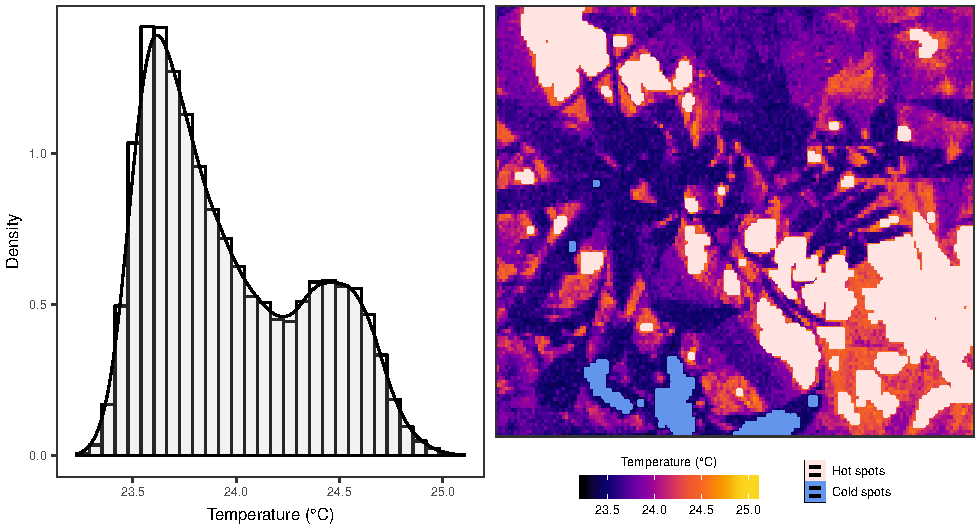
\includegraphics{./output/fig-B-1-1} 

}

\caption{The output of \texttt{plot\_patches} includes a histogram and the original temperature data overlaid with outlines of hot and cold spots, identified using the G* variant of the Getis-Ord local statistic.}\label{fig:fig-B-1}
\end{figure}

\pagebreak

\hypertarget{references}{%
\section*{References}\label{references}}
\addcontentsline{toc}{section}{References}

\hypertarget{refs}{}
\leavevmode\hypertarget{ref-faye_toolbox_2016}{}%
Faye, E., Rebaudo, F., Yánez-Cajo, D., Cauvy-Fraunié, S., \& Dangles, O. (2016). A toolbox for studying thermal heterogeneity across spatial scales: From unmanned aerial vehicle imagery to landscape metrics. \emph{Methods in Ecology and Evolution}, \emph{7}(4), 437--446. doi:\href{https://doi.org/10.1111/2041-210X.12488}{10.1111/2041-210X.12488}

\leavevmode\hypertarget{ref-getis_local_1996}{}%
Getis, A., \& Ord, J. K. (1996). Local spatial statistics: An overview. \emph{Spatial Analysis: Modelling in a GIS Environment}, \emph{374}, 261--277.

\leavevmode\hypertarget{ref-fragstats_2012}{}%
McGarigal, K., Cushman, S. A., \& Ene, E. (2012). FRAGSTATS v4: Spatial pattern analysis program for categorical and continuous maps. Retrieved from \url{http://www.umass.edu/landeco/research/fragstats/fragstats.html}

\leavevmode\hypertarget{ref-mcguire_achieving_2016}{}%
McGuire, J. L., Lawler, J. J., McRae, B. H., \& Theobald, D. M. (2016). Achieving climate connectivity in a fragmented landscape. \emph{Proceedings of the National Academy of Sciences}, \emph{113}(26), 7195--7200. doi:\href{https://doi.org/10.1073/pnas.1602817113}{10.1073/pnas.1602817113}

\leavevmode\hypertarget{ref-shi_framework_2016}{}%
Shi, H., Wen, Z., Paull, D., \& Guo, M. (2016). A framework for quantifying the thermal buffering effect of microhabitats. \emph{Biological Conservation}, \emph{204}, 175--180. doi:\href{https://doi.org/10.1016/j.biocon.2016.11.006}{10.1016/j.biocon.2016.11.006}

\leavevmode\hypertarget{ref-tattersall_thermimage:_2017}{}%
Tattersall, G. J. (2017). Thermimage: Thermal Image Analysis. Retrieved from \url{https://CRAN.R-project.org/package=Thermimage}

\leavevmode\hypertarget{ref-sdmtools_2014}{}%
VanDerWal, J., Falconi, L., Januchowski, S., Shoo, L., \& Storlie, C. (2014). SDMTools: Species distribution modelling tools: Tools for processing data associated with species distribution modelling exercises. Available at: \href{https://CRAN.R-project.org/package=SDMTools}{Https://cran.r-project.org/package=SDMTools}. Retrieved from \url{https://CRAN.R-project.org/package=SDMTools}


\end{document}
